\chapter*[Introdução]{Introdução}

    \addcontentsline{toc}{chapter}{Introdução}

    Em 1930, Alonzo Church, matemático estadunidense apresentou o Cálculo Lambda, como parte da investigação dos fundamentos da matemática. O Cálculo Lambda é um sistema que
    estuda funções recursivas computáveis e foi utilizada como base para as teorias e fundamentos matemáticos por trás do paradigma da Programação Funcional. Ele também
    pode ser considerado a primeira linguagem programação funcional, todavia, não foi projetada para ser executada em computadores, sendo apenas um modelo que descreve relações entre funções
    simples, permitindo criar funções mais complexas.

    Com o passar dos anos, varias linguagens funcionais foram criadas, sendo alguns exemplos a linguagem LISP em 1955 e a ML no final da década de 70. Porém, não
    havia um padrão para as linguagens desse paradigma, e quando chegou a segunda metade da década de 80, havia uma necessidade de criar uma única linguagem, que englobasse
    as melhores práticas de projeto, além de implementar as técnicas funcionais que estavam em alta na época.

    Nesse contexto Haskell foi criado em 1987, por Peyton Jones e Paul Hudak. Sendo assim a The Yale Meeting foi a primeira reunião presencial, no qual foi decidido
    os principais objetivos que a linguagem proporcionaria, como também a escolha do nome. 
    Segue as metas estabelecidas na reunião:

    \begin{itemize}
      \item Ser viável para o ensino, pesquisa e aplicações, incluindo sistema de larga escala;
      \item Ser completamente descritiva via publicação no tocante à sua sintaxe e sua semântica;
      \item Não ser proprietária, tal que qualquer um pudesse implementá-la e distribuí-la;
      \item Basear-se em ideias que envolvessem o senso comum;
      \item Reduzir a diversidade desnecessária de outras linguagens funcionais.
    \end{itemize} 

    A implementação de Haskell começou do zero, desenvolvendo funções únicas e tendo inspiração na linguagem Miranda que estava desempenhando um papel 
    importante na época. Em geral, essa linguagem passou por algumas versões que ajudou muito no desempenho e na adição de novas funções. 

    \newpage
    \chapter{Histórico sobre a linguagem, com sua cronologia}

    Depois desse evento, outras reuniões se sucederam e sendo assim no dia 01/04/1990, foi publicado primeiro relatório
    da versão 1.0 do Haskell. Durante os proximos 15 anos, Haskell teve o lançamento de diferentes versões, tranzendo outras
    funcionalidades para linguagem, entre elas se encontra Haskell'98 e Haskell 2010 que é sua versão mais recente.  

    O relatório da versão do Haskell'98 foi lançado em fevereiro de 1999. Ela surgiu no intuito de estabeler uma versão mais estável, 
    para ser possível realizar a documentação mais profunda da lingua em livros, já que o Haskell estava evoluindo muito rápido e ganhando 
    notoriedade.

    Em 2006 a equipe começou a planejar revisões anuais para adicionar o progresso do desenvolvimento da linguagem. Sendo assim a primeira revisão,
    publicada em julho de 2010, foi nomeada Haskell 2010 e nela foi incrementada uma serie recursos que antes não estavam disponiveis.
    Segue abaixo uma serie dos recursos que foram disponibilizados:
    
    \begin{itemize}
      \item Do and If Then Else 
      \item Hierarchical Modules
      \item Empty Data Declarations
      \item Fixity Resolution 
      \item Foreign Function Interface
      \item Line Comment Syntax
      \item Pattern Guards
      \item Relaxed Dependency Analysis
      \item Language Pragma
      \item Remove n+k patterns
    \end{itemize}

    Atualmente existem 3930 programadores com contas registradas que utilizam Haskell, sendo que 2566
    dessas contas são públicas e 1364 são privadas. Por causa do número de programadores, existem muitas 
    oportunidades nessa área, fazendo os empregos terem um sálario médio de \$80.000 à \$160.000.

    Por mais que Haskell não seja tão utilizado como antes, muitas aplicações foram feitas com a linguagem. 
    Algumas aplicações são:

    \begin{itemize}
      \item A biblioteca open-source Semantic, implementada pelo GitHub, foi puramente escrito em Haskell;
      \item O Facebook implementa programas anti-spam que são escritos em Haskell e são de código aberto;
      \item O Snap e Yesod, ambos frameworks para aplicações na web, foram feitos para suportar Haskell;
      \item O Linspire, sistema operacional comercial, tem Haskell como linguagem escolhida para o desenvolvimento das aplicações do sistema;
      \item Xmonad, totalmente escrito em Haskell, é um gerenciador de janela para o sistema X Window System.
    \end{itemize}

    \begin{figure}[ht]
        \centering
        \begin{tikzpicture}
            \begin{axis}[xbar interval, xmax=95,xmin=25, minor x tick num = 5]
              \addplot+[ 
              boxplot prepared={
                median=59.61,
                upper quartile=69.18,
                lower quartile=50.87,
                upper whisker=85.18,
                lower whisker=35.46
              },
              ] coordinates {};
            \end{axis}
        \end{tikzpicture}
        \caption{Box Plot}
    \end{figure}

    \begin{figure}[ht]
        \centering
        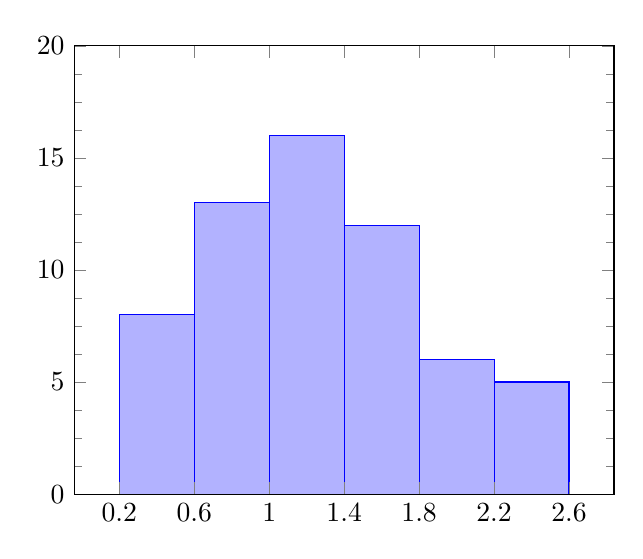
\begin{tikzpicture}
            \begin{axis}[
                ymin=0, ymax=20,
                minor y tick num = 3,
                area style,
                xtick = {0.2, 0.6,..., 2.6}
                ]
                \addplot+[ybar interval, mark=no] plot coordinates { (0.2, 8) (0.6, 13) (1.0, 16) (1.4, 12) (1.8, 6) (2.2, 5) (2.6, 5)};
            \end{axis}
        \end{tikzpicture}
        \caption{Histograma}    
    \end{figure}

    \nocite{haskellmicrosoft}
    \nocite{haskellreport2010}
    \nocite{haskelljobs}
    \nocite{haskellers}

    \newpage